\documentclass[10pt,DIV=15,twocolumn,ngerman,parskip=half]{scrartcl}
\usepackage{abstract}
\usepackage{babel}
\usepackage[tt=false]{libertine}
\usepackage[svgnames]{xcolor}
\usepackage[unicode=true,
            pdfstartview=FitH,
            pdfusetitle,
            colorlinks=true,
            allcolors=DarkBlue]{hyperref}
\usepackage{microtype}
\hypersetup{pdfauthor={Bernhard Walle, NCP engineering GmbH}}
\usepackage{listings}
\usepackage{graphicx}
\usepackage{lipsum}

\lstset{                   
       basicstyle=\footnotesize\ttfamily,
       tabsize=4,                                    
       showstringspaces=false,
       keywordstyle=\bfseries\color{blue!40!black},
       commentstyle=\color {green!40!black},
       numberstyle=\scriptsize\ttfamily, %
       numbers=none,
       frame=tb,
       breaklines=true,
       captionpos=b,
       breakindent=3pt,
       postbreak=\mbox{\textcolor{gray}{$\hookrightarrow$}\space},
  }
\usepackage[scale=.85]{sourcecodepro} 

\urlstyle{rm}

\begin{document}

\title{Linux-Fehleranalyse mit \emph{strace}}

\author{\href{mailto:bernhard.walle@ncp-e.com}{Bernhard Walle},
        \href{https://www.ncp-e.com}{NCP engineering GmbH}}

\date{14. Januar 2020}

\newcommand{\strace}{\emph{strace}}

\makeatletter
\twocolumn[
  \begin{@twocolumnfalse} 
    \maketitle 
    \begin{abstract} 
      Das Tool \strace{} gehört zu den Urgesteinen der Tracing"=Tools unter Linux und anderen
      unixoiden Betriebssystemen. Es ist entweder bereits installiert oder lässt sich über die
      Paketverwaltung leicht installieren. Mit Hilfe von \strace{} lässt sich die Interaktion
      eines beliebigen Programms mit dem Betriebssystem untersuchen: Es zeigt die sogenannten
      \emph{Systemaufrufe} mit ihren Argumente und Rückgabewerten an.

      Dieser Vortrag ist für Einsteiger gedacht und beginnt daher mit etwas Theorie: Wie
      interagieren Programme mit dem Betriebssystem? Danach wird die Bedienung von \strace{}
      anhand eines einfachen Beispiels erläutert. Zum Schluss folgen verschiedene nützliche
      Optionen mit ihren Einsatzszenarien.
    \end{abstract}

    \vspace{1cm}
  \end{@twocolumnfalse}
]
\makeatother

\section{Grundlagen}

\subsection{User-Mode und Kernel-Mode}

\begin{frame}
  \frametitle{User-Mode und Kernel-Mode}

  \begin{block}{Kernel-Mode}
    \begin{itemize}
      \item Zugriff auf gesamten Speicher und Hardware möglich
      \item auch als \emph{Supervisor-Modus} oder \emph{privilegierter Modus} bezeichnet
      \item wird nur vom Kernel verwendet
    \end{itemize}
  \end{block}

  \begin{block}{User-Mode}
    \begin{itemize}
      \item eingeschränkter Befehlssatz
      \item verwenden normale Programme, auch als Root
    \end{itemize}
  \end{block}
\end{frame}

\subsection{Systemaufrufe}

\begin{frame}
  \frametitle{Systemaufrufe}

  \begin{block}{Was sind Systemaufrufe?}
    Systemaufrufe ermöglichen einem Programm, Dienste des Betriebssystems in Anspruch zu nehmen,
    die den \emph{Kernel-Mode} erfordern.
  \end{block}
  
  \begin{block}{Gruppen von Systemaufrufen}

    \begin{itemize}
      \item Datei- und Verzeichnisverwaltung
      \item Prozessmanagement
      \item Speicherverwaltung
      \item Interprozesskommunikation (IPC)
      \item Netzwerkkommunikation
      \item Behandlung von Signalen
      \item Sonstiges
    \end{itemize}
  \end{block}

\end{frame}

\begin{frame}
  \frametitle{Systemaufrufe für Dateioperationen}

  \begin{itemize}
    \item \texttt{open()} 
      \begin{itemize}
        \item öffnet Datei
        \item gibt \emph{Dateideskriptor} zurück
        \item erwartet Dateinamen und Zugriffsmodus als Parameter
      \end{itemize}

    \item \texttt{read()}
      \begin{itemize}
        \item liest Inhalt von einer Datei
        \item bekommt \emph{Dateideskriptor} (und Speicher) als Argument
        \item gibt Anzahl gelesener Bytes zurück
      \end{itemize}

    \item \texttt{close()}
      \begin{itemize}
        \item gibt Dateideskriptor wieder frei
      \end{itemize}

  \end{itemize}
\end{frame}

\begin{frame}
  \frametitle{Dateideskriptoren}

  \begin{block}{Bedeutung}
    \begin{itemize}
      \item identifiziert geöffnete Datei
      \item Zahl, innerhalb eines Prozesses eindeutig
      \item auch für andere Objekte, insb. \emph{Sockets} (für Netzwerkkommunikation)
    \end{itemize}
  \end{block}

  \begin{block}{Vordefinierte Dateideskriptoren}
    \centering
    \medskip
    \begin{tabular}{|lll|}
      \hline
      \textbf{Dateideskriptor} & \textbf{Symbol} & \textbf{Bedeutung} \\
      \hline
        0      & \texttt{STDIN}    & Standardeingabe (Tastatur) \\
        1      & \texttt{STDOUT}   & Standardausgabe (Terminal) \\
        2      & \texttt{STDERR}   & Standardfehlerausgabe (Terminal) \\
      \hline
    \end{tabular}
    \medskip
  \end{block}
\end{frame}

\begin{frame}
  \frametitle{Parameter und Rückgabewerte}

  \begin{block}{Parameter}
    \begin{itemize}
      \item Zahl und Typ abhängig vom konkreten Systemaufruf
      \item dokumentiert in der jeweiligen Manpage
    \end{itemize}
  \end{block}

  \begin{block}{Rückgabewert}
    \begin{itemize}
      \item immer eine Zahl
      \item $\ge$ 0: Bedeutung abhängig vom Systemaufruf
      \item $<$   0: Fehlercode
      \begin{itemize}
        \item vordefinierte Werte (POSIX, Linux-spezifisch)
        \item dokumentiert in \href{http://man7.org/linux/man-pages/man3/errno.3.html}{\emph{errno(3)}} 
        \item kleine Auswahl auf der nächsten Folie
      \end{itemize}
    \end{itemize}
  \end{block}


\end{frame}

\begin{frame}
  \frametitle{Auswahl verbreiter Fehlercodes}

  \bigskip\centering
  \begin{tabular}{|r@{~~}l|l|}
    \hline
    \multicolumn{2}{|l|}{\textbf{Fehlercode}}        & \textbf{Bedeutung} \\
    \hline
    -1      & \texttt{EPERM}     & Die Operation ist nicht erlaubt \\
    -2      & \texttt{ENOENT}    & Datei oder Verzeichnis nicht gefunden \\
    -5      & \texttt{EIO}       & Eingabe-/Ausgabefehler \\
    -13     & \texttt{EACCES}    & Keine Berechtigung \\
    -20     & \texttt{ENOTDIR}   & Ist kein Verzeichnis \\
    -21     & \texttt{EISDIR}    & Ist ein Verzeichnis \\
    -28     & \texttt{ENOSPC}    & Auf dem Gerät ist kein Speicherplatz mehr verfügbar \\
    \hline
  \end{tabular}


\end{frame}

\begin{figure*}[t]
  \centering

  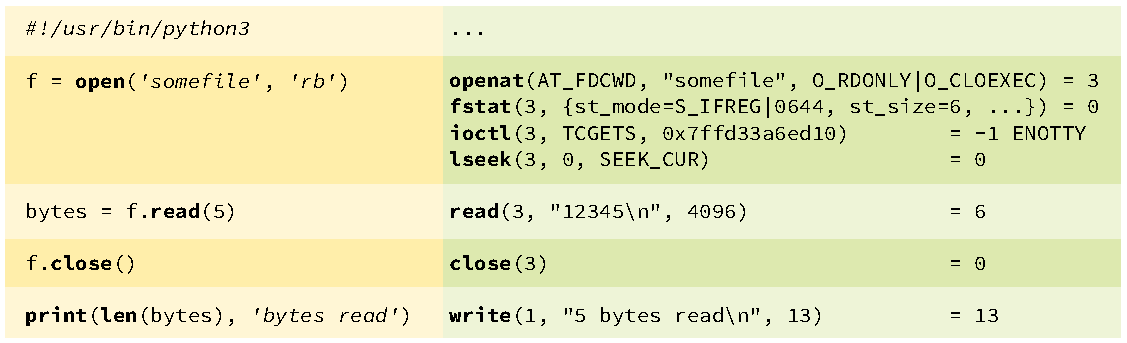
\includegraphics[scale=.8]{../images/sample-listing}
  \caption{Beispielhaftes Python-Programm (link) und dessen \strace-Ausgabe (rechts) \newline
  \emph{Anmerkung:} Die \strace-Ausgabe wurde um den relevanten Anteil gekürzt
  }
  \label{fig:sample-listing}
\end{figure*}

\section{\strace{} in Aktion}

\subsection{Analyse eines einfachen Programms}
\label{sec:simpleprogram}

Genug der Theorie. In diesem Abschnitt wollen wir uns die Ausgabe von \strace{} anhand eines
einfachen Beispiels ansehen. \autoref{fig:sample-listing} zeigt links ein kurzes Python-Skript.
Python wurde deshalb gewählt, weil es auch ohne Spezialkenntnisse leicht verständlich ist --
deutlich einfacher als die Programmiersprache C.

Ein Shellskript ist zur Darstellung von \strace{} ungeeignet, da es in der Regel sehr viele externe
Programme aufruft, sog. \emph{Kindprozesse}. Gerade zu Beginn eines neu gestarteten Programmes
werden jedoch viele Systemaufrufe durchgeführt (Laden von Bibliotheken, Übersetzungsdateien),
die für Laien erstmal schwer verständlich sind.


Auf der rechten Seite von \autoref{fig:sample-listing} wird die unveränderte Ausgabe von \strace{}
dargestellt. Allerdings wurde nur der wesentliche Teil gelistet.

Um das Beispiel nachvollziehen zu können, starten wir das Programm folgendermaßen in einer Shell:

\begin{lstlisting}
  % strace notfound.py > output.txt
\end{lstlisting}

Die Ausgabeumleitung in \texttt{output.txt} wird vorgenommen, damit sich die Ausgabe vom Programm
und von \strace{} nicht vermischen. Zunächst werden einige hundert Zeilen Output erzeugt, die für
uns irrelevant sind. Bevor der Python-Interpreter das Programm ausführt, muss erst eimal der
Python-Interpreter initialisiert werden, müssen Bibliothken vom Betriebssystem geladen werden und
muss das eigentliche Skript gelesen werden. Bei einem kompilierten C-Programm wäre dieser Anteil deutlich kürzer aber dennoch relativ groß.

Die Kunst besteht darin, den eigentlichen Start des Teils des Programms zu finden, der uns
interessiert. Am besten liest man von unten nach oben. Oder man leitet die Ausgabe von \strace{}
ein eine Datei um -- wie das geht erfahren wir im nächsten Kapitel -- und sucht im Texteditor nach
einem bekannten String: Das kann eine (bekannte) Ausgabe sein oder der Namen der Datei, die
geöffnet wird.

Das Beispiel wurde so formatiert, dass die Zeilen des Programms und die korrespondierenden
Systemaufrufe klar erkennbar sind. Dennoch nachfolgend ein paar Erklärungen.

Zunächst wird die Datei \texttt{somefile} zum Lesen geöffnet. Daraus resultiert ein Systemaufruf
\texttt{open()}. Der Python-Interpreter verwendet das etwas modernere \texttt{openat()}, welches
zusätzlich noch ermöglicht, anzugeben, wie relative Pfade behandelt werden.

Das Ergebnis ist der \emph{Dateideskriptor} mit der Nummer 3, der bei den folgenden Systemaufrufen
dann immer als erstes Argument angegeben wird. Dieser Dateideskriptor ist wichtig um die Aufrufe
den verschiedenen Dateien zuordnen zu können!

Anschließend werden Metainformationen zur Datei gelelesen, dafür wird \texttt{fstat()} verwendet.
Zur Metainformation gehören die Größe und Zugriffsrechte der Datei. Der Aufruf \texttt{ioctl()}
prüft, ob die Datei ein Terminal ist, \texttt{lseek()} setzt die Position des Lesezeigers auf den
Anfang.

\notebox{\sffamily
      Im Prinzip sind diese Operationen für das Programm gar nicht erforderlich.
      Das ist ein
      Problem der Abstraktion in der Informatik: Je "`einfacher"' die Programmiersprache gehalten
      ist, je mehr automatisch passiert, deso schwieriger wird es, das Verhalten des Systems auf
      unterster Ebene zu verstehen und deso mehr Dinge werden erledigt, die gar nicht erledigt
      werden müssten.}

Nun werden mit \texttt{f.read()} maximal 5 Bytes gelesen. Der Python-Interpreter hingegen puffert
intern, versucht also einen ganzen Puffer von 4096 Bytes zu lesen und bekommt tatsächlich 6 Bytes.
Dies ist der Rückgabewert des Systemaufrufs \texttt{read()}.

\texttt{close()} gibt den Dateideskriptor 3 wieder frei. \texttt{write()} schreibt die Meldung "`5
Bytes read"' auf die Standardausgabe. Gemäß \autoref{tab:errno} ist der Dateideskriptor 1 die
Standardausgabe.

\minisec{Fehlerfall}

Nun löschen wir die Datei \texttt{somefile,} so dass sie nicht vorhanden ist\footnote{Deshalb heißt
das Programm ja auch \texttt{notfound.py}.} und starten das Programm erneut. Die wesentliche
Zeile der \strace-Ausgabe sieht wie folgt aus:

\begin{lstlisting}
openat(AT_FDCWD, "somefile", O_RDONLY|O_CLOEXEC) = -1 ENOENT (Datei oder Verzeichnis nicht gefunden)
\end{lstlisting}

Hier ist klar erkennbar, dass die Datei nicht geöffnet wurde, weil die nicht exisistiert. Statt
einem (positiven) Dateideskriptor gibt \texttt{openat()} den Fehlercode $-1$ zurück, der gemäß
\href{http://man7.org/linux/man-pages/man3/errno.3.html}{\emph{errno(3)}} bzw. \autoref{tab:errno}
„Datei oder Verzeichnis nicht gefunden“ bedeutet. Dieser Fehlertext ist praktischerweise in der
Ausgabe von \strace{} auch gleich mit enthalten.

Danach kommen jede Menge Fehlerausgaben, die einfach deshalb in \strace{} auftauchen, weil sich das
Python-Programm mit einer Ausnahme beendet.

\subsection{Kindprozesse und Threads}

\strace{} verfolgt standardmäßig nur den direkt gestarteten Prozess und den
Haupt-Thread\footnote{Ein \emph{Thread} (von engl. \emph{thread} = „Faden“) ist ein
Ausführungsstrang eines Programms. Mit Hilfe von Threads können Programme mehrere Dinge parallel
erledigen ohne dass damit verschiedene, komplett getrennte Prozesse gestartet werden müssen. Somit
können die Threads alle auf die gleichen Daten zugreifen.}.

Aus Betriebssystemsicht (unter Linux) sind Threads und Kindprozesse\footnote{Vereinfacht gesagt:
Wenn aus einem Programm ein anderes gestartet wird, nennt man den neu entstehenden Prozess
\emph{Kindprozess.}} ziemlich ähnlich, nämlich sog. \emph{Scheduling-Einheiten}. Trotzdem haben
alle Threads innerhalb des gleichen Prozesses die gleiche Prozess-ID (PID), aber eine andere
Thread-ID (TID). Leider verwendet \strace{} aus historischen Gründen die Terminologie "`PID"', meint
aber eigentlich die TID.

Aufgrund dieser Verwandtschaft von Threads und Prozessen gibt es in \strace{} auch nur eine Option:
Startet man \strace{} mit der Option \texttt{-f} (für \emph{follow),} werden auch Kindprogramme und
andere Threads beobachtet. Die Ausgabe wird jedoch schnell unübersichtlich -- wie man etwas Abhilfe
schafft beschreibt \autoref{sec:fileoutput}.

Um die Programme unterscheiden zu können beginnt jede Trace-Zeile eines Kindprozesses mit
\texttt{[pid XXXX]}, wobei \texttt{XXXX} für die jeweilige Prozess-ID bzw. Thread-ID steht.


\subsection{Protokollierung in eine Datei}
\label{sec:fileoutput}

Wie wir in \autoref{sec:fileoutput} gesehen haben, wird die Ausgabe von \strace{} mit der des
eigentlichen Programms vermischt. Zwar schreibt \strace{} auf die Standardfehlerausgabe, jedoch
kann auch das zu beobachtenden Programm die Fehlerausgabe benutzen. Daher helfen Ausgabeumleitungen
der Shell nicht weiter. Stattdessen kann mit der Option \texttt{-o \emph{Dateiname}} die gesamte
Ausgabe von \strace{} in \texttt{\emph{Dateiname}} umgeleitet werden.

Wird beim Tracen von Kindprozessen statt \texttt{-f} die Option \texttt{-ff} angegeben, erstellt
\strace{} pro PID eine eigene Datei nach dem Schema \texttt{\emph{Dateiname}.\emph{PID}}. Das macht
das Lesen übersichtlicher. Um die Systemaufrufe auch zeitlich einordnen zu können, kann man
\strace{} mit \texttt{-t} anweisen, die aktuelle Systemzeit in die Protokolliertung hinzuzufügen,
mit \texttt{-tt} auch in der Genauigkeit von Millisekunden. Die Protokollierung von Zeitstempeln
ist unabhängig davon, ob die Ausgabe in eine Datei umgeleitet wird oder nicht.

\subsection{Filterfunktionen}

Die vorhergehenden Abschnitte haben durch neue Optionen die Ausgabe immer noch angereichert, was
zwar nützlich ist, aber das Ganze nicht unbedingt übersichtlicher macht. In diesem Abschnitt wollen
wir den Output etwas einschränken.

Meistens interessiert man sich nicht für das Verhalten des Programms als Ganzes sondern für einen
bestimmten Teilaspekt. So könnte uns beispielsweise interessieren, warum eine Datei nicht geöffnet
werden kann. Relevant ist also eigentlich nur der \texttt{open}-Systemaufruf.

Zur Einschränkung gibt es die Option \texttt{-e trace=\emph{set}}; \texttt{\emph{set}}
steht dabei für einen oder mehrere Systemaufrufe, jeweils durch Kommata getrennt.

Nun ist es meistens eine schlechte Idee, \strace{} auf einen genauen Systemaufruf einzuschränken.
Im konkreten Beispiel (warum wird eine Datei nicht gefunden) lauern zwei Fallen: Erstens wurde
\texttt{open()} mittlerweile bei aktuellen C"=Bibliotheken durch \texttt{openat()} ersetzt, zweitens
könnte das Programm vor dem Öffnen mit \texttt{stat()} prüfen, ob die Datei überhaupt existiert.

Deshalb gibt es vordefinierte Gruppen, nämlich \texttt{\%file} für Dateioperationen.
\autoref{tab:strace_groups} liefert die wichtigsten Gruppen für Systemaufrufe.


\begin{figure*}[tb]
  \lstinputlisting[numbers=left,xleftmargin=3em,stepnumber=2]{../sample/strace_file_ls.txt}
  \caption{Einschränkung von \strace{} auf Dateioperationen}
  \label{fig:fileonly}
\end{figure*}


\begin{table}[htb]
  \centering\small
  \begin{tabular}{|lp{6cm}|}
    \hline
    \textbf{Gruppe} & \textbf{Operationen} \\
    \hline
    \texttt{\%file}          & Dateioperationen, die einen Dateinamen als Argument
                               bekommen, also beispielsweise \texttt{open,} \texttt{stat,}
                               \texttt{chmod,} \texttt{unlink,} … \\
    \texttt{\%desc}          & Dateioperationen, die einen Dateideskriptor als Argument
                               bekommen, also z.\,B. \texttt{read,} \texttt{write,}
                               \texttt{chmod,} \texttt{unlink,} … \\
    \texttt{\%process}       & Systemaurufe zur Prozessverwaltung \\
    \texttt{\%net}           & Systemaurufe zur Netzwerkprogrammierung \\
    \texttt{\%signal}        & Systemaurufe bzgl. Behandlung von Signalen \\
    \texttt{\%ipc}           & Operationen zur Interprozesskommunikation \\
    \texttt{\%memory}        & Systemaufrufe zur Speicherverwaltung \\
    \texttt{\%pure}          & Systemaufrufe ohne Argument, z.\,B. \texttt{getpid} \\
    \hline
  \end{tabular}
  \caption{Gruppen von Systemcalls für \texttt{-e trace=\emph{group}}}
  \label{tab:strace_groups}
\end{table}

Ein Beispiel: \autoref{fig:fileonly} zeigt die \emph{vollständige} Ausgabe von \texttt{strace -e
trace=\%file ls}. Ohne diese Einschränkung wäre das Listing 66 Zeilen lang! Zunächst werden
die Biblitoheken und Übersetzungsdateien geladen, anschließend wird in Zeile 9 dann der
Dateideskriptor für das aktuelle Arbeitsverzeichnis geöffnet. Zeile 10 und 11 sind bereits
die eigentliche Ausgabe des Programms.

Es gibt noch wesentlich mehr Möglichkeiten der Filterung, die in der Manpage
\href{http://man7.org/linux/man-pages/man1/strace.1.html#OPTIONS}{\emph{strace(1)}} im Abschnitt
„Options“ und weiter unter „Filtering“ detailliert beschrieben werden.

\subsection{Strings}

Der Übersichtlichkeit halber schneidet \strace{} längere Strings ab, beispielsweise bei Texten, die
mit \texttt{write} ausgegeben werden. Der Schalter \texttt{-s \emph{LÄNGE}} erlaubt es dem
Benutzer, eine deutlich längere Maximalgröße für Strings festzulegen. Dateinamen werden nie
abgeschnitten.

\section{Vorhandene Prozesse}

Bisher haben wir \strace{} immer mit einem Programm von Anfang an gestartet. Aber oftmals
ist es auch nützlich, \strace{} auf bereits laufende Prozesse loszulassen, um beispielsweise zu
sehen warum ein Programm hängt.

Zunächst müssen wir dafür die Prozess-ID (PID) des Prozesses herausfinden, entweder mit
\texttt{pidof} oder mit \texttt{ps}. Anschließend kann sich \strace{} mit \texttt{-p \emph{PID}}
an den laufenden Prozess anhängen. Die Option \texttt{-f} (mehrere Threads/Kindprozesse) gilt
analog.

\minisec{Berechtigungen}

Allerdings darf man natürlich nur die Prozesse des eigenen Benutzers verfolgen, nur der
Root-Benutzer darf fremde Tasks tracen. Die Standardkonfiguration vieler Linux-Distributionen
verbietet es allerdings, dem normalen Benutzer fremde Prozesse zu verfolgen. Diese Einstellung
kann mit folgendem Befehl (temporär) geändert werden:

\begin{lstlisting}
  % sudo sysctl kernel.yama.ptrace_scope=0
\end{lstlisting}

Unter \cite{yama} ist diese Einstellung dokumentiert. Über einen Eintrag in
\href{http://man7.org/linux/man-pages/man5/sysctl.conf.5.html}{\emph{sysctl.conf(5)}} kann man
diese Einstellung auch persistent anwenden.


\minisec{Dateideskriptoren zuordnen}

Läuft der Prozess bereits, fehlen einem die entsprechenden \texttt{open()}-Aufrufe, um zu wissen,
welcher Dateideskriptor zu welcher Datei gehört. Diese Information bekommt man leicht aus dem
Proc-Dateisystem: Pro Prozess-ID existiert in \texttt{/proc} ein Verzeichnis, mit jeweils einem
Unterverzeichnis \texttt{fd} (für \emph{file descriptor}). Dort existiert wiederum für jeden
numerischen Dateideskriptor ein symbolischer Link, der zur tatsächlichen Datei zeigt.

Am besten betrachten wir ein Beispiel, nämlich wieder unser leicht modifizertes Programm
\texttt{notfound.py} aus \autoref{fig:sample-listing}. Es wurde lediglich zwischen dem Öffnen
und Schließen der Datei eine kleine Wartezeit eingefügt.

Zunächst finden wir mit \texttt{ps aux|grep notfound.py} die PID des Programms heraus, anschließend
erzeugen wir ein Verzeichnislisting mit \texttt{ls -l /proc/\emph{PID}/fd}:

\begin{lstlisting}
lrwx------ 1 bw bw 64  2. Jan 16:35 0 -> /dev/pts/1
lrwx------ 1 bw bw 64  2. Jan 16:35 1 -> /dev/pts/1
lrwx------ 1 bw bw 64  2. Jan 16:35 2 -> /dev/pts/1
lr-x------ 1 bw bw 64  2. Jan 16:35 3 -> /home/bw/devel/strace-talk/sample/somefile
\end{lstlisting}

0, 1 und zwei sind jeweils mit Standardein-, -ausgabe und -fehlerausgabe vorbelegt (vgl.
\autoref{tab:stdio} während der Dateideskriptor 3 auf die vom Programm selbst geöffnete Datei zeigt.

\tipbox{Mit dem Schalter \texttt{-y} kann diese Arbeit auch \strace{} für uns übernehmen. Bei jedem
Dateideskriptor wird zusätzlich in spitzen Klammern die zugehörige Datei mit dargestellt!}



\vfill

\begin{thebibliography}{99}
  \bibitem{tanenbaum}
    \textsc{Tanenbaum, Andrew S.}: \emph{Moderne Betriebssysteme}. 3., aktualisierte Auflage. :
     Pearson Studium, 2009. \newline
     ISBN 3827373425 
   \bibitem{manstrace} Manpage
    \href{http://man7.org/linux/man-pages/man1/strace.1.html}{\emph{strace(1)}}
 \end{thebibliography}

\end{document}